%Kapitel der Umsetzung

\chapter{OSINT einer ausgewählten Person}  %Name des Kapitels
\label{cha:Informationsbeschaffung einer ausgewählten Person} %Label des Kapitels

\section{Auswahl der Programmiersprache}
Damit das Programm anhand den Lösungsideen umgesetzt werden kann, ist der erste Schritt die Auswahl der Programmiersprache.\\
Hierbei wird keine Anforderung an die Geschwindigkeit der Sprache gestellt, da beim web scraping das Internet den zeitlichen Engpass darstellt. Allerdings wäre es von Vorteil wenn bereits entwickelte Bibliotheken für das OSINT vorhanden sind. Die Eingabe der Information für die Suche kann über eine Konsole oder über eine graphische Benutzeroberfläche möglich sein.\\
Als mögliche Programmiersprachen zählen Python, Ruby, C++.\\
Für web-basierende Anwendung eignet sich eine dynamische Programmsprache.
Im Gegensatz zu Python und Ruby zählt C++ nicht zur Familie der dynamischen Programmiersprachen und fällt aus diesem Grund als mögliche Lösung heraus. \\
Python und Ruby können beide Webseiten, die JavaScript zum rendern benötigen, laden. Dies ist mit Hilfe eines automatisierten Webbrowsers möglich. Des Weiteren lässt sich die Anwendung durch beide Sprachen, entsprechend den Anforderungen entwickeln. Es kann sowohl eine Oberflächenanwendung als auch eine Konsolenanwendung programmiert werden. Zusätzlich bringen beide Sprachen Module mit sich, um das Pojekt mit den vorgegebenen Zielen umzusetzen. Somit haben beide Programmiersprachen die Voraussetzungen für die Entwicklung der Anwendung. Allerdings bietet Python in diesem Bereich eine große Community und eignet sich sehr gut für die Bearbeitung von linguistischen Daten. \cite{bird2009natural}
Aus diesen Gründen wird die zu erstellende Anwendung mit der Programmiersprache Python entwickelt.
	
\section{Methoden zur Suche nach einer Person im Internet}
\label{sec:Suche nach Information}
Die Art der Personensuche wird abhängig von den eingegeben Daten  variiert. Das heißt, dass die eingegebenen Daten über die Zielperson vor der Suche analysiert werden und dementsprechend angepasst wird. Nachstehen werden zwei grundsätzliche Methoden für die Art der Personensuche beschrieben.

	\subsection{Personensuche mit Hilfe einer Suchmaschine}
	\label{subsubsec:PersonensucheMitHilfevonSuchmaschine}
	Hier wird mit Hilfe einer Suchmaschine nach Informationen gesucht. Mögliche Suchmaschinen sind die von Google und Bing. Allerdings muss nicht für jede Suche eine Suchmaschine verwendet werden. Die nachfolgenden Fälle sollen diesen Ansatz verdeutlichen.
	
	Im Fall, dass der Vorname, Nachname und Wohnort der gesuchten Person eingegeben wird, kann mit Hilfe der festgelegten Suchmaschine nach Information gesucht werden. Die von der Suchmaschine vorgeschlagenen Seiten werden anschließend analysiert, ausgelesen und gespeichert. Dadurch können weitere Informationen gewonnen werden. Falls Benutzernamen von anderen Webseiten wie Instagram, Facebook oder ähnliches vorgeschlagen werden, kann somit die Suche mit diesen Daten speziell auf den entsprechenden Seiten erweitert werden.
	
	Ein weiterer Fall beschreibt das Szenario, wenn ein Benutzername der gesuchten Person in das Programm eingegeben wird. Hierbei handelt es sich um einen Benutzernamen von Social-Media-Webseiten wie Facebook, Instagram, LinkedIn, et cetera. \\
	Zuallererst, wird hier nach Einträgen auf der entsprechende Webseite zu dem angegebenen Benutzername gesucht. Dadurch können zusätzliche Daten herausgefunden werden. Diese sind bei der weiteren Suche von Vorteil.\\
	Sobald die Webseite mit Hilfe des Nutzernamens durchsucht und ausgewertet wurde, kann die Suche mit einer Suchmaschine und den gewonnen Daten erweitert werden.
	
	\subsection{Personensuche auf festgelegten Webseiten}
	\label{subsubsec:PersonensucheohneSuchmaschine}
	Unabhängig von den eingegebenen Daten, wird eine festgesetzte Anzahl von Webseiten durchsucht. Als potentielle Kandidaten-Webseiten eigenen sich die Social-Media-Seiten wie Facebook, Instagram, Twitter, LinkedIn, et cetera. Diese Art der Personensuche arbeitet allerdings ohne die Verwendung einer Suchmaschine.
	
\section{Bewertung der Methoden zur Personensuche}
Um möglichst viele Informationen über eine Person im Internet zu finden, bietet die Personensuche mit der Verwendung einer Suchmaschine die beste Lösung. Es wird anstatt ausschließlich festgelegten Seiten das ganze Internet durchsucht. Dadurch können wesentlich mehr individuelle Einträge gefunden werden. Des Weiteren wird keine Logik zur Suche nach Einträgen im Internet benötigt, da lediglich den vorgeschlagenen Suchergebnissen gefolgt werden kann.\\
Allerdings muss beachtet werden, dass Benutzer bei verschiedensten Social-Media-Seiten auswählen können, ob das Benutzerprofil von einer Suchmaschine gefunden werden kann oder nicht. Bekannte Webseiten die diese Einstellungsmöglichkeiten unterstützen sind XING und LinkedIn. Aus diesem Grund, werden zu Beginn der Suche die Social-Media-Seiten durchsucht. Dadurch können vor der Google-Suche zusätzliche Informationen herausgefunden werden, die für das später OSINT von Vorteil sind. Falls sich eine Social-Media-Seite unter den Google-Suchergebnissen befindet, kann diese nachträglich ebenfalls durchsucht werden.

	\subsection{Auswahl der Suchmaschine}
	Laut Expertenaussage sucht Bing tiefgreifender nach Information auf Social Media Seiten wie Facebook, Twitter und LinkedIn. Allerdings finden nur 3,5\% aller Suchanfragen in Deutschland über Bing statt. Im Gegensatz dazu hat Google einen Marktanteil von 91,2\% in Deutschland. Diese Zahlen sprechen eindeutig für Google. Durch die höhere Anzahl von Suchanfragen, können mehr Daten erfasst und die Ergebnislisten besser gerankt werden. Dies hat zu Folge, dass Bing bei einer konkreten Suche schlechter abschneidet. \cite{Suchmaschinen}
	Grundsätzlich stellt die Verwendung von zwei Suchmaschinen die beste Lösung dar, da die Wahrscheinlichkeit für einen Suchtreffer erhöht wird. Dennoch wird in dieser Arbeit ausschließlich die Suchmaschine von Google verwendet, da sie gegenüber dem Konkurrenten keine Nachteile hat. Selbst die detailliertere Suche auf Sozialen Netzwerken, bringt bei der hier verwendeten Personensuche keinen großen Vorteil für Bing. Das heißt, durch die Analyse der Suchergebnisse, wird erkannt ob sich die bekannten Social Media Webseiten darunter befinden. Falls diese es nicht tun, wird die Suche auf den entsprechenden Sozialen Netzwerken erweitert.
	 	
\section{Umsetzung: Personensuche mit Hilfe der Google-Suchmaschine im Internet}
Die Suchmaschine von Google wird für die Personensuche im Internet verwendet. Gesucht wird nach den eingegebenen Daten, welche über die Konsole eingelesen werden.

	\subsection{Eingabe der bekannten Daten}
	Es besteht die Möglichkeit den \textbf{Vorname, Nachname, Wohnort, Arbeitgeber, Instagram Benutzername, Facebook Benutzername, Twitter Benutzername, E-Mail-Adresse}, und das genaue beziehungsweise geschätzte \textbf{Geburtsjahr} der gesuchten Person über eine Konsole einzugeben. Falls der genaue Jahrgang der Zielperson nicht bekannt ist, kann ein geschätztes Geburtsjahr eingetragen werden. Dies kann später bei der Identifizierung der gesuchten Person hilfreich sein.\\
	Zu Beginn werden alle Personen-Variablen mit einem leeren String initialisiert. Das bedeutet, alle Variablen, zu denen keine Information eingegeben wurde, enthalten einen leeren String.
	
		\subsubsection{Verarbeitung der Daten}
		Im ersten Schritt wird kontrolliert, welche Informationen vom Progamm-Nutzer eingegeben wurden. Der Vorname und Nachname sind nicht ausreichend für die Suche. Es wird mindestens ein weiteres Attribute benötigt. Dagegen ist der Benutzernamen von Instagram und Twitter sowie die E-Mail-Adresse einzigartig. Dadurch kann mit einem dieser Attribute gesucht werden.\\
		Bei der Eingabe des Wohnortes, kann dieser vor der Suche mit der entsprechenden Wortsammlung verglichen werden. Falls sich der Wohnort nicht in der Datenbank befindet, wird er nachträglich ergänzt. Für die Personenerkennung ist es wichtig, dass sich der korrekt Wohnort in der Datenbank befindet.\\
		Daraufhin werden mit diesen Eingaben Kombinationen für die Suche und die URL-Generierung erstellt. Mögliche Such-Kombinationen für erfolgreiche Ergebnisse sind:
		
		\textit{Vorname, Nachname, Wohnort;}\\
		\textit{Vorname, Nachname, Geburtsjahr;}\\
		\textit{Vorname, Nachname, Institution;}\\
		\textit{Vorname, Nachname, Wohnort, Geburtsjahr;}\\
		\textit{Vorname, Nachname, Wohnort, Institution;}\\
		\textit{Benutzername einer Social-Media-Seite;}
		
		
		Die Kombination aus vielen oder allen Daten ist ebenfalls eine mögliche Option. Allerdings wird dadurch oft kein Ergebnis gefunden, da nicht zur jeder Information ein Eintrag im Internet besteht.\\
		Sobald die Kombinationen aus den Daten bekannt sind, werden die Such-URLs für die Google-Suchmaschine generiert.
		\subsection{Generierung der Google-Such-URLs}
			\subsubsection{Aufbau eines URLs}
			\label{subsec:AufbauURL}
			Ein Uniform Resource Locator (URL) lokalisiert eine Ressource, indem eine abstrakte Identifikation der Lokalisierung verwendet wird. Dabei wird ein URL grundsätzlich im folgenden Format angegeben.\cite{RFC1738}
			
			$<scheme>:<scheme-specific-part>$ \cite{RFC1738}
			
			Das Schema gleicht hierbei meist dem verwendeten Protokoll wie HTTP oder FTP. Der Doppelpunkt stellt die Trennung zum Schema-spezifischen Teil dar. Ein Beispiel für ein HTTP-URL-Aufbau ist im Folgenden definiert.\cite{RFC1738}
			
			$http://<host>:<port>/<path>?<searchpart>$\cite{RFC1738}
			
			Hier wird das Protokoll HTTP als Schema verwendet, wobei sich der Aufbau bei der Verwendung des HTTPS-Protokolls kaum unterscheidet. Lediglich das Schema und der Port verändert sich.\\
			Für den <host> kann der FQDN oder die IP-Adresse des Hostrechners eingetragen werden. Wenn der Port nicht angegeben wird, ist der Standardport voreingestellt. Bei HTTP wäre dies Port 80 und bei HTTPS Port 443. Der <path> stellt ein HTTP-Selektor dar und ist mit einem Fragezeichen von der Suchzeichenkette getrennt.\cite{RFC1738}\\ %TODO FQDN in Abkürzungsverzeichnis	
			Im Bereich des <searchpart> lassen sich URL-Parameter einfügen um Informationen an die entsprechende Webseite mitzugeben. Die Parameter bestehen aus einem Schlüssel und aus einem Wert, welche durch ein Gleichheitszeichen getrennt werden. Um mehrere Parameter hinzuzufügen und zu kombinieren wird das kaufmännische Und-Zeichen verwendet.\cite{GoogleURL}\\
			Ein URL für die Google-Suche von \textit{Max Mustermann} ist in dem folgenden Beispiel gegeben.
			
			$https://www.google.com/search?q=Max+Mustermann$
			%TODO Möglicherweise zeichnung mit Beschriftung wie bei wikipedia
			
			Allerdings können URLs nur mit ASCII-Zeichen erzeugt und versendet werden. Aus diesem Grund müssen Zeichen die nicht im ASCII vorkommen, in ein gültiges Format umgewandelt werden. Dies wird realisiert, indem die URL-Kodierung das nicht enthaltende ASCII-Zeichen durch ein "'\%"', gefolgt von zwei Hexadezimalen Ziffern, ersetzt. Beispielsweise repräsentiert "'\%20"' ein Leerzeichen und "'\%22"' ein Anführungszeichen. \cite{HTMLURL} \\
			
			\subsubsection{Erstellen der Such-URLs}
			Dieser Absatz beschreibt die Erstellung der Such-URLs für Google, mit dem Wissen aus Kapitel \ref{subsec:AufbauURL}.\\
			Für jede genannte Kombination aus den eingegebenen Daten werden Link-Muster erzeugt. Diese entsprechen einem Lückentext. Sobald die entsprechenden Muster ausgewählt wurden, werden die Lücken mit den Daten befüllt. Dadurch wird eine Liste mit einer variierende Menge von Suchlinks erstellt. Diese Liste wird anschließende von dem Web Crawler verwendet um die Suche zu starten.
			Ein URL für die Suche nach Information auf beliebigen Webseiten wird wie folgt dargestellt.
			
			\textit{https://www.google.com/search?q=\%22Max+Mustermann\%22+\%22Weingarten\%22}
			
			Wenn allerdings der Benutzername einer Social-Media-Seite bekannt ist, werden zwei unterschiedliche URLs verwendet. Mit Hilfe des ersten URLs, wird speziell nach Einträgen auf der entsprechenden Webseite gesucht. Dazu kann der Operator "'site"' verwendet werden. Dieser beschränkt die Suchergebnisse soweit, dass die vorgeschlagenen Einträge ausschließlich auf einer festgelegten Webseite vorkommen. Das folgende Beispiel beschreibt die Suche nach dem Benutzer "'Mustermann"' auf der Webseite "'Instagram.com"'. Dabei ersetzt die ASCII-Zeichenkette "'\%3A"' den Doppelpunkt. \cite{HTMLURL}
			
			\textit{https://www.google.com/search?q=site\%3Ainstagram.com+\%22Mustermann\%22}
			
			Der zweite URL wird für eine Social-Media-Suche verwendet. Bei dieser Suche werden Social-Media-Seiten nach Einträgen durchsucht. Dafür wird kein zusätzlicher Operator benötigt. Es wird lediglich ein @-Zeichen, welches mit der Zeichenkette "'\%40"' dargestellt wird, vor dem zu suchenden Wort eingefügt. Die Social-Media-Suche nach dem Benutzernamen "'Mustermann"' sieht folgendermaßen aus.\cite{SocialMediaSearch}
			
			\textit{https://www.google.de/search?q=\%40Mustermann}
			
			\subsubsection{Optimierung der Such-URLs}
			\label{subsubsec:URLOptimieren}
			Um die Suchergebnisse von Google zu verbessern, können die Suchbegriffe in Anführungszeichen gesetzt werden. Dadurch wird eine Phrasensuche gestartet, die nach einer Zeichenfolge sucht. Das bedeutet, es wird ausschließlich nach diesen Zeichenfolgen gesucht und nicht nach einer Abwandlung. Ein Beispiel hierfür ist die Suche nach "'Mike Bazzell"'. Wenn diese Suche ohne Anführungszeichen durchgeführt wird, werden zusätzlich Webseiten vorgeschlagen die den Namen Mike Bazzell anstatt Micheal Bazzell beinhalten. Diese erweiterte Suche kann dazu führen, dass unzählige Webseiten vorgeschlagen werden, die nicht unbedingt was mit dem Thema der Suchbegriffe zu tun hat. Um dem vorzubeugen können Anführungszeichen verwendet werden, welche die Anzahl der Suchergebnisse um einen sehr großen Teil verringern. \cite{Bazzell}\\
			Für die Suche nach \textbf{Marco Lang} werden ungefähr \textbf{96.400.000} Ergebnisse mit Hilfe der Google-Suchmaschine gefunden. Wird die Suche mit den Anführungszeichen verfeinert indem nach \textbf{"'Marco"' "'Lang"'} gesucht wird, werden etwa \textbf{55.600.000} Ergebnisse gefunden. Allerdings werden hier Webseiten vorgeschlagen, welche die Wörter "'Marco"' und "'Lang"' beinhalten, jedoch müssen diese nicht direkt nebeneinander und auch nicht in der Reihenfolge vorkommen. Es wäre Möglich, dass bei dieser Suche, Webseite mit Verweisen auf die Namen "'Marco Mustermann"' und "'Max Lang"' beinhaltet. Aus diesem Grund kann nach \textbf{"'Marco Lang"'} gegoogelt werden. Dadurch wird die Anzahl der Suchergebnisse auf \textbf{45.500} Ergebnisse reduziert. Der Grund für die starke Reduzierung ist, dass ausschließlich die Webseiten vorgeschlagen werden, die den kompletten String "'Marco Lang"' beinhalten. Für eine weitere Optimierung der Ergebnisse, wird der Wohnort hinzugefügt, wie in dem Beispiel \textbf{"'Marco Lang"' "'Tettnang"'}. Dadurch werden die Suchvorschläge auf lediglich \textbf{95} Ergebnisse reduziert. Die URL zu dieser optimierten Suche lautet: 
			
			\textit{https://www.google.com/search?q=\%22Marco+Lang\%22+\%22Tettnang\%22}
			
			Nicht nur die Reduzierung der Suchergebnisse, sondern auch das herausfiltern von unerwünschten Webseiten hat einen positiven Effekt auf die zu erstellende Anwendung, da die vorgeschlagenen Seiten in den folgenden Schritten analysiert werden müssen. Das bedeutet, dass jede unerwünschte Seite die allein durch die Suche herausgefiltert werden kann, einen großen Laufzeitvorteil mit sich bringt. 
			
			
		
		\subsection{Mit welcher Bibliothek werden Serveranfragen umgesetzt?}
		Damit eine Person im Internet gesucht werden kann, muss das Programm in der Lage sein, Anfragen an einen Server zu versenden und die dazugehörigen Antwort zu empfangen. \\
		Im Folgenden werden drei Möglichkeiten beschrieben, um Anfragen an einen Server zu versenden. Zum einen ist das die Python Request-Bibliothek, welche sich optimal für HTTP-Anfragen eignet.\cite{WebScraping} Zum anderen bietet sich die Verwendung eines automatisierten Webbrowsers an, was mit Hilfe der Selenium Python API realisierbar ist.\cite{lawson2015web} Über diese API ist es möglich auf alle Funktionen des Selenium WebDrivers zuzugreifen.\cite{SeleniumWithPython} Eine Alternative dazu, ist das Python Framework Scrapy, welches zum Crawlen von Webseiten und Extrahieren von Daten verwendet werden kann.\cite{Scrapy} Die letzte Möglichkeit stellt die  Scrapy Middleware Scrapy-Selenium dar.\cite{scrapy-selenium} Dadurch wird die Kommunikation von Scrapy und Selenium ermöglicht.
		
		Für komplizierte Anfragen an einen Server eignet sich die Request-Bibliothek von Python sehr gut. Der Umgang mit Cookies, Header und vielem mehr ist sehr einfach gestaltet. Auch die Generierung des Such-URLs wird von dieser Bibliothek übernommen. Des Weiteren hat Requests einen großen Laufzeit-Vorteil gegenüber dem automatisierten Webbrowser und kann HTTP-Fehlermeldungen empfangen. Allerdings lässt sich mit der Request-Bibliothek keine Javascript-Seite auslesen.\\
		Wenn das Framework Scrapy standardmäßig verwendet wird, können ebenfalls keine Javascript-Seiten ausgelesen werden. Doch in Scrapy lässt sich ein automatisierter Webbrowser einfügen, mit welchem das Auslesen von Javascript-Webseiten möglich ist. Zusätzlich lässt sich mit Scrapy ein effektiver Web Crawler und Web Scraper entwickeln, was für die nächsten Schritte ein erheblicher Vorteil ist.\\
		Aus den erläuternden Gründen, wird das Framework Scrapy mit der Verbindung eines automatisierten Webbrowsers für die Personensuche verwendet. Der automatisierte Webbrowser muss in dem Framework implementiert werden, da auf bestimmte Webseiten mit Javascript direkt zugegriffen wird. Infolgedessen wird die Middelware Scrapy-Selenium verwendet, da sie die eine kompakte Möglichkeit bietet, den automatisierten Webbrowser in Scrapy zu implementieren. Durch diese Kombination aus Scrapy und dem Selenium WebDriver, lassen sich Javascript-Seiten problemlos auslesen. \\
		Zusätzlich zu diesem Framework wird ein unabhängiger Selenium-Wedriver implementiert. Dieser wird für den Umgang mit den Social-Media-Seiten benötigt, da auf diesen Seiten ein Login vollzogen werden muss. Das hat den Vorteil, dass die Anmeldung in der Session gespeichert wird. Somit muss bei einem erneuten Zugriff auf die selbe Seite keine neue Anmeldung vollzogen werden.
	
		\subsection{Web Crawler erstellen}
		%TODO Muss Scrapy und Selenium erklärt werden?

		Nachdem der Selenium WebDriver in das Scrapy Framework implementiert wurde, kann mit dem crawling begonnen werden. Der Web Crawler hat die Aufgabe ausgewählte Social-Media-Seiten zu durchstöbern und den von Google vorgeschlagenen Webseiten zu folgen. Wie in Bild \ref{img:AufbauWebCrawler} gezeigt, werden zuerst die Informationen über die Zielperson eingelesen. Anschließend werden die Social-Media-Seiten behandelt, wodurch weitere Informationen über die Person gefunden werden können. Die bekannten Informationen über die gesuchte Person, werden zur Generierung der Google-Such-Links verwendet. Mit diesen Links und der Hilfe von der Google-Suchmaschine, werden Webseiten gesucht, die mögliche Inhalte betreffend der Zielperson enthalten. Im nächsten Schritt wird die Google-Webseite mit den Suchergebnissen analysiert und ausgelesen. Dadurch können die URLs für die entsprechenden Webseiten gewonnen werden. Diesen URLs wird anschließend gefolgt, um Informationen über die Zielperson zu gewinnen.\\
		
		\begin{figure}[H]
			\centering
			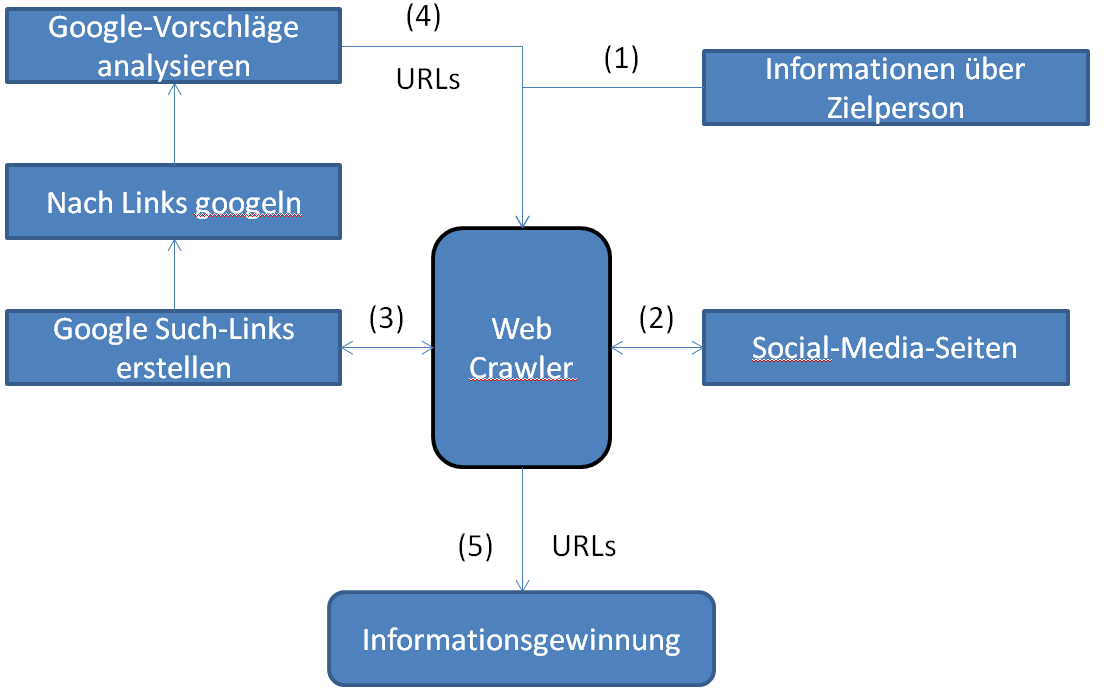
\includegraphics[ scale=0.5]{bilder/webcrawler.PNG}
			\caption{Aufbau des Web Crawlers}
			\label{img:AufbauWebCrawler}
		\end{figure}
		%TODO Bild ohne roten Linien einfügen
		
			\subsubsection{Social-Media-Seiten}
			\label{subsubsec:SocialMediaSeiten}
			Zu den verwendeten Social-Media-Webseiten gehören Instagram, Facebook, Twitter, Xing und LinkedIn. Für diese Webseiten werden Fake-Accounts und ein eigener Selenium WebDriver erstellt. Dieser automatisierte Webbrowser ist ausschließlich für die Social-Media-Seiten zuständig. Damit vollständige Profile angezeigt werden können, loggt sich dieser automatisch ein. Die gewonnen Informationen werden dem Profil der gesuchten Person hinzugefügt und zusätzlich für die Google-Suche verwendet.\\
			Es kann passieren, dass ausschließlich der Benutzername von einer Person bekannt ist. Weiter Attribute wie Vorname, Nachname und Wohnort sind nicht bekannt. In dem Fall, kann mit einem einzigartigen Benutzername nach diesen Attributen auf der entsprechenden Webseite gesucht werden. Jedoch verwendet nur Instagram und Twitter ein einmaligen Benutzernamen. Aus diesem Grund kann die erweiterte Suche nur auf diesen beiden Plattformen umgesetzt werden.
			
			\textbf{Login-Formulare}\\
			Der Selenium WebDriver muss sich nicht bei jeder Social-Medi-Webseite einloggen. Zu beginn wird kontrolliert, zu welcher Plattform ein Benutzername eingegeben wurde. Dazu gibt es bei dieser Anwendung die Möglichkeit einen Facebook-, Instagram- oder Twitter-Benutzername einzugeben. Je nach Eingabe meldet sich der Browser auf den entsprechenden Seiten an. Auf den Seiten Xing und LinkedIn wird sich standardmäßig  angemeldet. Das hat den Grund, dass diese beiden Seiten immer durchsucht werden sollen. \\
			Bei der Umsetzung wird im ersten Schritt die Login-Seite der entsprechenden Plattform angefordert. Die Antwort wird mit Hilfe der BeautifulSoup-Bibliothek nach dem HTML-Tag <input> durchsucht. Allerdings hat nicht jede Webseite den komplett identischen Aufbau. Das bedeutet, dass sich bei diesen Tags die Attribute unterscheiden können. Aus diesem Grund muss nach der Angeforderten-Webseite die Suche der <input>-Tags unterschieden werden.\\
			Die Anmeldung von Instagram, Facebook und LinkedIn sind nahezu identisch. Hier können die zwei gesuchten <input>-Felder mit Hilfe des Attributs \textit{type} identifiziert und gefunden werden. Bei der Twitter-Login-Seite muss anstatt dem \textit{type} nach dem Attribute \textit{class} gesucht werden. Andernfalls findet der Browser keine interaktiven Elemente.\\
			Zum übertragen der Benutzernamen und Passwörter, benötigt der Selenium WebDriver ein Element mit eindeutigem Attribut zur Referenzierung. Dafür dient bei Instragram, LinkedIn und Facebook das vorher gefundene Element mit dem Attribute "'id"'. Bei Twitter ist das dass Attribut "'class[0]"' und bei Xing "'name"'.
			 
			\textbf{Instagram}\\
			Instagram und Twitter verwenden beide einen einzigartigen Benutzername. Dies ist ein riesigen Vorteil für die Identifikation einer Person, wenn der Benutzername bekannt ist. Allerdings ist es ebenfalls möglich eine Person mit ihrem offiziellen Namen zu suchen und zu finden.\\
			Im Fall, dass der Instagram-Benutzername eingegeben wurde, wird die dazugehörige Profilseite angezeigt und nach Informationen durchsucht. Im nächsten Schritt dienen die vorgeschlagenen Freunde, welche in Beziehung zu diesem Profil stehen, als weitere Informationsquelle. Das bedeutet, dass diese Kontakte ebenfalls durchsucht werden. Bei Übereinstimmungen wie zum Beispiel der selben Universität, kann später eine glaubwürdige Phishing-Mail generiert werden.\\
			Falls sich jedoch eine Instagram-Seite unter den Google-Vorschlägen befindet, und die Übereinstimmung des Profils mit der Zielperson nicht klar ist, können die Vorgeschlagenen Kontakte für die Identifizierung der Zielperson genutzt werden. So wird beispielsweise erkannt, wenn ein Freunden aus der selben Stadt vorgeschlagen werd, dass es sich um die gesuchte Person handeln kann. Diese Methode erzielt kein sicheres Ergebnis. Jedoch kann die Wahrscheinlichkeit erhöht werden, dass es sich um die richtige Person handelt.\\
			Die Profilseite wird mit dem folgenden Link \textit{https://www.instagram.com/username/} angefordert. Weitere Seiten und Einträge der gesuchten Person, unabhängig von der Profilseite,können mit dem Suchbefehl \textbf{site:instagram.com "'username"' \\ -site:instagram.com/username} angezeigt werden. \cite{Bazzell} In der Anwendung wird dies mit dem folgenden URL umgesetzt.
					
			\textit{https://www.google.com/search?q=site\%3Ainstagram.com+\%22username\%22+-site\\
				\%3Ainstagram.com\%2Fusername\&oq=site\%3Ainstagram.com+\%22username\%22+-site\\
				\%3Ainstagram.com\%2Fusername}
			
			Die dazugehörigen Suchergebnisse werden anschließend gleich den normalen Google-Suchergebnissen behandelt.
			
			\textbf{Twitter}\\
			Auf der Webseite Twitter wird ausschließlich die Profilseite nach Informationen durchsucht. Dies ist mit dem Link \textbf{https://twitter.com/username} möglich.
			
			\textbf{Facebook}\\
			Facebook bietet ein großes Potential um OSINT zu betreiben. Allerdings hat Facebook optimal Algorithmen zur Erkennung von automatisierten Crawlern entwickelt. Aus diesem Grund wurde das Fake-Konto nach wenigen Versuchen gesperrt. Das hat zu Folge, dass auf dieser Plattform nur begrenzt gesucht werden kann, da keine Anmeldung vorgenommen wird. Um das Konto zu entsperren müssten eine Kopie des Ausweises, ein Bild mit erkennbarem Gesicht und eine Handynummer an Facebook übermittelt werden.\\
			Aus diesen Gründen wird Facebook nur dann und ohne Anmeldung verwendet, wenn sich ein Vorschlag unter den Google-Suchergebnissen befindet.

			\textbf{LinkedIn und XING}\\
			LinkedIn und XING bieten eine optimale Informationsquelle bezüglich der schulischen und beruflichen Laufbahn der Zielperson. Allerdings gibt es hier keinen einzigartigen Benutzernamen. Demzufolgem, wird eine Person mit dem vollen Namen und dem aktuellen Wohnort gesucht. Dabei wird auf LinkedIn ein Filter angewendet, bei dem ausschließlich Personen aus Deutschland angezeigt werden. Wenn genau eine Person vorgeschlagen wird, wird dieses gefundene Personenprofil durchsucht. Bei einer Mehrzahl von gefunden Personen werden diese nicht auf Informationen durchsucht, da keine Identifikation möglich ist.\\
			Die Personensuche bei LinkedIn, mit angwandtem Filter, wird mit dem URL\\ \textit{https://www.linkedin.com/search/results/people/?facetGeoRegion=\%5B\%22de\%3A0\%22\%5D\\
				\&keywords=vorname\%20nachname\%20wohnort\&origin=FACETED\_SEARCH} dargetellt. \\
			Bei Xing sieht der Such-URL wie folgt aus.\\			
			\textit{https://www.xing.com/search/old/members?hdr=1\&keywords=vorname+nachname++wohnort}
			
			
			\subsubsection{Webseite mit den Suchergebnissen von Google analysieren}
			Zur Analyse der Webseite mit den Suchergebnissen von Google, wird der Seitenquelltext benötigt. Mit Hilfe des Quelltextes, können  die entsprechenden Links erkannt werden. Der Seitenquelltext wird mit Hilfe der BeautifulSoup-Bibliothek angezeigt.\\
			Das Bild \ref{img:GoogleSuchergebnis} stellt ein Suchergebnis von Google dar. Der dazugehörige Quelltext befindet sich in der Darstellung \ref{lst:GoogleSeitenquelltext}.
			\begin{figure}[H]
				\centering
				
\includegraphics[ scale=0.65]{bilder/Google-Suchergebnis1.png}
				\caption{Google-Suchergebnis \cite{suchergebnisseMarco}}
				\label{img:GoogleSuchergebnis}
			\end{figure}
			Im Ausschnitt des Seitenquelltextes \ref{lst:GoogleSeitenquelltext} ist zu sehen, dass der <div>-Container mit der Klasse "'g"' einen Hyperlink enthält. URLs oder Links werden mit dem HTML-Tag <a> dargestellt. Dieser Link wird für die Suche benötigt. Deswegen wird genau nach diesem Link gesucht.\\
			Da der <div>-Container bei jedem Suchergebnis identisch ist, kann bei jedem Ergebnis nach dem entsprechenden <div>-Container gesucht werden. Anschließend kann der erste Link in diesem <div>-Tag ausgelesen werden. Dies wird mit Hilfe der BeautifulSoup-Bibliothek umgesetzt.\\ %TODO DIE oder DER URL
			Um zu erkennen, ob mehrere Seiten mit Suchergebnissen existieren, wird nach bestimmten Hyperlinks gesucht. Diese Links werden über das Attribute "'class"' identifiziert. Mit Hilfe der BeautifulSoup-Bibliothek wird nach dem Klassennamen "'fl"' gesucht. Falls weiter Seiten mit Suchergebnissen vorhanden sind, werden die dazugehörigen Links in einer Liste gespeichert. Anschließend wird ihnen gefolgt und die neue Seite wird nach weiteren URLs durchsucht.\\
			%TODO sollen wirklich mehrere Seiten durchsucht werden???\\
		
			\begin{lstlisting}[caption=Ausschnitt des Quelltextes von einem einem Google-Suchergebnis \cite{suchergebnisseMarco},label={lst:GoogleSeitenquelltext}]
			<div class="g">
				<h3 class="r">
					<a href="/url?q=https://www.fupa.net/spieler/marco-lang
						-1261543.html&amp;sa=U&amp;ved=0ahUKEwiZ3PDGqMvhAhWt
						URUIHU7VAcwQFggUMAA&amp;usg=AOvVaw2QiSMFzScB0Jcvo
						PCisBGw"><b>Marco Lang</b>- Spieler - FuPa - FuPa
					</a>
				</h3>	
			\end{lstlisting} 

\section{Methoden zum Erkennen von wichtigen Informationen auf einer Webseite}
\label{subsec:ErkennenVonInformation}
Bei der Suche nach einer ausgewählten Person können verschiedenste Arten von Webseiten gefunden werden. Aus diesem Grund muss das Programm eine gewisse Intelligenz mit sich bringen um die wichtigsten Daten aus einer Seite herauszufiltern. Dabei ist es nicht möglich eine Hartkodierung zu verwenden, um festgelegte Bereiche einer Webseite auszulesen, da jede Webseite eine individuelle Struktur hat.\\
Die Grundidee zur Lösung diese Problems ist die Analyse des vorliegenden Webseiten-Textes. Eine Methode zur Textanalyse ist die automatisierte Schlüsselwort-Gewinnung. Hierbei wird die HTML-Seite zu einem verwendbaren Text formatiert, wobei alle Sonderzeichen herausgefiltert werden. Für die E-Mail-Erkennung wird der unformatierte Text verwendet, da Sonderzeichen wie "'."' und "'@"'  dabei von Nöten sind. Im nächsten Schritt werden Schlüsselwörter aus dem formatierten Webseitentext generiert. Möglichkeiten zur automatisierten Schlüsselwortgenerierung sind die Verfahren RAKE \ref{sec:RAKE} und die Automatic Keyword Extraction mit NLP \ref{sec:Automatic Keyword Extraction}, welche im Laufe dieser Arbeit detailliert beschrieben werden.\\
Nachdem die Schlüsselwörter generiert und in Listen gespeichert wurden, werden Wortsammlung erstellt. Diese Wortsammlungen sind Listen, welche aussagekräftige Schlüsselwörter enthalten und nach Themen kategorisiert sind. Beispiele für den Inhalt der Listen sind alle Hochschulen und Universitäten in Deutschland, Berufsbezeichnungen und Tätigkeiten, Studiengänge, Hobbybezeichnungen und alle Städte und Gemeinden in Deutschland.\\
Mit diesen Wortsammlungen kann nun die Liste mit den bereits generierten Schlüsselwörtern aus dem Webseitentext verglichen werden. Bei einer Übereinstimmung eines Schlüsselwortes wird das Wort mit der entsprechenden Kategorie vorgemerkt und später in die verwendete Speicherstruktur eingetragen. \\
Die Wortsammlungen werden mit Hilfe von bekannten Listen im Internet eigenständig befüllt. Als Informationsquelle dienen alle öffentlich frei zugänglichen Listen, die hilfreiche Informationen enthalten.

	\subsection{RAKE}
	\label{sec:RAKE}
	RAKE steht für \textit{Rapid Automatic Keyword Extraction} und stellt eine sehr effiziente Methode zur Schlüsselwortgenerierung dar. Die Funktion von RAKE basiert darin, dass Schlüsselwörter mehrere Wörter mit inhaltlicher Relevanz enthalten, allerdings selten Stoppwörter und Sonderzeichen.\cite{rose2010automatic}\\
	Als Stoppwörter werden Wörter bezeichnet, die sehr oft auftreten und keinen großen Informationsgewinn mit sich bringen. Beispiele dafür sind \textit{und}, \textit{weil}, \textit{der} oder \textit{als}.\cite{Stopwords}\\
	
	\begin{figure}[h!]
		\fbox{\parbox{\linewidth}{In einer jungen Wissenschaft wie der Informatik mit ihrer Vielschichtigkeit und ihrer unüberschaubaren Anwendungsvielfalt ist man oftmals noch bestrebt, eine Charakterisierung des Wesens dieser Wissenschaft und Gemeinsamkeiten und Abgrenzungen zu anderen Wissenschaften zu finden. Etablierte Wissenschaften haben es da leichter, sei es, dass sie es aufgegeben haben, sich zu definieren, oder sei es, dass ihre Struktur und ihre Inhalte allgemein bekannt sind.}}
		\caption{Beispieltext \cite{schubert2011didaktik}}
		\label{fig:text}
	\end{figure}
	
	Zu Beginn wird der zu analysierende Text, hier der Beispieltext in  Bild \ref{fig:text}, durch einen Worttrenner in ein Array, bestehen aus möglichen Schlüsselwörtern, aufgeteilt. Das erzeugte Array wird anschließend in Sequenzen von zusammenhängenden Wörtern unterteilt. Dabei erhalten die Wörter in einer Sequenz die gleiche Position und Reihenfolge wie im Ursprungstext und dienen gemeinsam als Kandidatenschlüsselwort.\cite{rose2010automatic}\\		
	Nachdem die möglichen Schlüsselwörter identifiziert sind, wird für jeden einzelnen Kandidaten ein Score ausgerechnet. Dieser besteht aus dem Quotient des Grades $deg(w)$ und der Häufigkeit des Vorkommens eines Wortes innerhalb der Kandidaten $freq(w)$. Daraus ergibt sich die Formel:
	\begin{center}
		$deg(w)/freq(w) $
	\end{center}	
	
	Dabei beschreibt der Grad eines Wortes, dass gemeinsame Auftreten mit sich selbst und anderen Schlüsselwörtern. In der Tabelle \ref{tab:Co-occurance} ist der Grad für jedes Wort ablesbar, indem die Einträge in der entsprechenden Reihe summiert werden. Beispielsweise Beträgt der Grad des Wortes \textit{"'Wissenschaft"'} den Wert \textit{3}. Dies ergibt sich aus der Rechnung:
	\begin{center}
		$2 + 1 = 3$
	\end{center}
	Das Wort \textit{"'Wissenschaft"'} kommt hier selbst zweimal in dem Kandidaten-Array vor und davon einmal in Verbindung mit dem Worten "'jungen"'.\\
	Die Häufigkeit des Vorkommens eines Wortes lässt sich ebenfalls in der Tabelle \ref{tab:Co-occurance} ablesen. Allerdings muss hier in der Reihe und Spalte des jeweiligen Wortes nachgeschaut werden. Für das Wort \textit{"'Wissenschaft"'} beträgt die Häufigkeit des Vorkommens den Wert \textit{3}.\\
	Zusammenfassend kann gesagt werden, dass \textit{deg(w)} die Kandidaten bevorzugt, welche oft und in langen Schlüsselwörtern, die mehrere Wörter enthalten, vorkommen. Dies bedeutet, dass beispielsweise \textit{deg(etabliert)} eine höhere Bewertung als \textit{deg(informatik)} bekommt, obwohl beide Wörter gleich oft im Text vorkommen. Dagegen wird bei \textit{freq(w)}, ausschließlich die Häufigkeit des Vorkommens bewertet. Bei der Formel \textit{deg(w)/freq(w)} werden die Wörter bevorzugt, welche überwiegend in langen Kandidatenwörtern vorkommen. Diese Formel bietet dadurch einen guten Mittelweg zur Schlüsselwortgewinnung. Ein Beispiel dafür sind die Wörter \textit{"'Wissenschaften} und \textit{"'allgemein"'}. Hier ist der Quotient von \textit{deg(allgemein)/freq(allgemein)} höher als von \textit{deg(Wissenschaften)/freq(Wissenschaften)}, obwohl die Häufigkeit des Wortes \textit{"'Wissenschaften"'} höher und der Grad gleich hoch ist. \cite{rose2010automatic}
	
	Durch das genannte Verfahren und der Formel \textit{deg(w)/freq(w)} für die Bewertung, ergeben sich die im Bild \ref{fig:SchlüsselwörterMitScore} befindenden Kandidaten mit den dazugehörigem Endbewertungen. \cite{rose2010automatic}
	
	\begin{center}
		\begin{table}[h!]
			\scriptsize
			\begin{tabular}{*{24}{l|}}				
				\rotatebox[origin=c]{90}{} 
				&\rotatebox[origin=c]{90}{wissenschaften} &\rotatebox[origin=c]{90}{wissenschaft} &\rotatebox[origin=c]{90}{sei} &\rotatebox[origin=c]{90}{etablierte} &\rotatebox[origin=c]{90}{informatik} &\rotatebox[origin=c]{90}{aufgegeben} &\rotatebox[origin=c]{90}{gemeinsamkeiten} &\rotatebox[origin=c]{90}{oftmals} &\rotatebox[origin=c]{90}{charakterisierung} &\rotatebox[origin=c]{90}{jungen} &\rotatebox[origin=c]{90}{inhalte} &\rotatebox[origin=c]{90}{allgemein} &\rotatebox[origin=c]{90}{bekannt} &\rotatebox[origin=c]{90}{struktur} &\rotatebox[origin=c]{90}{wesens} &\rotatebox[origin=c]{90}{bestrebt} &\rotatebox[origin=c]{90}{unüberschaubaren} &\rotatebox[origin=c]{90}{anwendungsvielfalt} &\rotatebox[origin=c]{90}{definieren} &\rotatebox[origin=c]{90}{abgrenzungen}
				&\rotatebox[origin=c]{90}{leichter}
				&\rotatebox[origin=c]{90}{finden}
				&\rotatebox[origin=c]{90}{vielschichtigkeit}\\
				\hline
				wissenschaften & 2 & & & 1 & & & & & & & & & & & & & & & & & & &\\
				\hline
				wissenschaft & & 2 & & & & & & & & 1 & & & & & & & & & & & & & \\
				\hline
				sei & & & 1 & & & & & & & & & & & & & & & & & & & &	\\
				\hline
				etablierte & 1 & & &1 & & & & & & & & & & & & & & & & & & &	\\
				\hline
				informatik & & & & &1 & & & & & & & & & & & & & & & & & & \\
				\hline
				aufgegeben & & & & & &1 & & & & & & & & & & & & & & & & &	\\
				\hline
				gemeinsamkeiten & & & & & & & 1& & & & & & & & & & & & & & & &	\\
				\hline
				oftmals & & & & & & & & 1& & & & & & & & & & & & & & &\\
				\hline
				charakterisierung & & & & & & & & & 1& & & & & & & & & & & & & & \\
				\hline
				jungen & & 1 & & & & & & & & 1 & & & & & & & & & & & & &	\\
				\hline
				inhalte & & & & & & & & & & & 1 & 1 & 1 & & & & & & & & & &	\\
				\hline
				allgemein & & & & & & & & & & & 1 & 1 & 1 & & & & & & & & & & \\
				\hline
				bekannt & & & & & & & & & & & 1 & 1 & 1 & & & & & & & & & &	\\
				\hline
				struktur & & & & & & & & & & & & & &1 & & & & & & & & &	\\
				\hline
				wesens & & & & & & & & & & & & & & &1 & & & & & & & &\\
				\hline
				bestrebt & & & & & & & & & & & & & & & & 1& & & & & & & \\
				\hline
				unüberschaubaren & & & & & & & & & & & & & & & & & 1 & 1 & & & & &	\\
				\hline
				anwendungsvielfalt & & & & & & & & & & & & & & & & & 1 & 1 & & & & &	\\
				\hline
				definieren & & & & & & & & & & & & & & & & & & & 1 & & & & \\
				\hline
				abgrenzungen & & & & & & & & & & & & & & & & & & & & 1 & & &	\\
				\hline
				leichter & & & & & & & & & & & & & & & & & & & & & 1 & &	\\
				\hline
				finden & & & & & & & & & & & & & & & & & & & & & & 1 & \\
				\hline
				vielschichtigkeit & & & & & & & & & & & & & & & & & & & & & & & 1	\\
				\hline
			\end{tabular}
			\label{tab:Co-occurance}
			\caption{Co-occurance}
		\end{table}
	\end{center}
	
	\begin{figure}[h!]
		\fbox{\parbox{\linewidth}{ inhalte allgemein bekannt (9.0), unüberschaubaren anwendungsvielfalt (4.0), jungen wissenschaft(3.5), etablierte wissenschaften (3.5), wissenschaften (1.5), wissenschaft (1.5), wesens (1.0), vielschichtigkeit (1.0), struktur (1.0), sei (1.0), oftmals (1.0), leichter (1.0), informatik (1.0), gemeinsamkeiten (1.0), finden (1.0), definieren (1.0), dass (1.0), charakterisierung (1.0), bestrebt (1.0), aufgegeben (1.0), abgrenzungen (1.0)}}
		\caption{Schlüsselwörter mit zugehörigem Score}
		\label{fig:SchlüsselwörterMitScore}
	\end{figure}
	\FloatBarrier

	\subsection{Automatic Keyword Extraction mit NLP}
	\label{sec:Automatic Keyword Extraction}
	Bei dieser Methode wird der vorliegende Text in die einzelnen Wörter unterteilt. Dabei wird eine Liste mit potentiellen Schlüsselwörtern erstellt, in der \textit{Stoppwörter} und Sonderzeichen herausgefiltert werden. Bei den Schlüsselwörtern handelt es sich nicht ausschließlich um ein Wort sondern auch um Wortsequenzen. Sogenannte N-Gramme bestehen aus einer festgelegten Anzahl von Wörtern. Dies hat den Vorteil, dass nicht nur Schlüsselwörter bestehend aus einem Wort erstellt werden können, sondern auch Schlüsselwörter mit Fragmenten eines Textes. Diese Art von Schlüsselwort wird benötigt um Informationen wie \textit{Hochschule Ravensburg-Weingarten} herauszulesen.\\
	Erweiternd kann die Anzahl der Schlüsselwörter mit dem Verfahren von Stemming reduziert werden. Durch die Verwendung von ergänzende Regeln wie, eine Mindestanzahl von Buchstaben in einem Wort, können die Schlüsselwörter weiter begrenzen.

 

\section{Bewertung der Methoden zum Herausfiltern von wichtigen Informationen auf einer Webseite}
RAKE stellt eine fertige Methode dar, um Schlüsselwörter, die den Inhalt eines Textes in kurz wiedergeben, zu erstellen. Dabei hat ein Anwender kaum Möglichkeiten eigene Implementierungen vorzunehmen, da vieles vorgegeben ist. In der zu erstellenden Anwendung soll jedoch nicht der Inhalt eines Textes in Schlüsselwörter zusammengefasst werden, sondern es wird nach informationsreichen Wörtern gesucht. Aus diesem Grund ist jedes einzelne Wort aus dem Webseiten-Text von Bedeutung. Dies spricht gegen RAKE, da es nur die selbst errechnenden Favoriten-Schlüsselwörter zur Verfügung stellt. Dadurch werden viele Wörter nicht in Betracht gezogen oder für weiterführende Bearbeitungen nicht bereitgestellt. Darüber hinaus ist die Berechnung eines Scores für diese Anwendung nicht notwendig.\\
Die Methode zur automatisierten Schlüsselwortgenerierung mit NLP bringt dagegen ein eigene Implementationsmöglichkeit mit sich. Das bedeutet, es kann selbst festgelegt werden, aus wie vielen Wörtern die Schlüsselwörter bestehen sollen. Des Weiteren wird jedes einzelne Wort in Betracht gezogen und verwendet.\\ Die Suche nach einer E-Mail-Adresse im Text lässt sich bei beiden Methoden hinzufügen. Jedoch wird aus den eben genannten Vorteilen, die Information mit Hilfe der Methode zur automatisierten Schlüsselwortgewinnung mit NLP herausgefiltert.


\section{Implementierung der Methoden zum Herausfiltern von wichtigen Informationen auf einer Webseite}
	\subsection{Text formatieren}
	\label{subsec:TextFormatieren}
	Bevor die Schlüsselwörter generiert werden können, muss der Text in ein verwertbares Format umgewandelt werden. Aus diesem Grund wird der Seitenquelltext zuallererst mit Hilfe des Python-Skripts html2text zu einem ASCII Plaintext umgewandelt.\cite{html2text} Anschließend werden Zeilenumbrüche und Sonderzeichen aus diesem Text herausgefiltert. Einzelne Wörter und Zahlen die weniger als 2 Zeichen beinhalten, werden ebenfalls aussortiert. Nachdem der Text in ein verwertbares Format umgewandelt wurde, kann mit der Umsetzung für die automatisierte Schlüsselwortgenerierung mit NLP begonnen werden.
	
	\subsection{Wortsammlungen erstellen}
	Die Ausführlichkeit der Wortsammlungen ist sehr wichtig für das Projekt, da die Informationsgewinnung abhängig von diesen Listen ist. Das bedeutet, umso besser diese Datenbanken erstellt werden, umso mehr Informationen können gewonnen werden.
	
		\subsubsection{Erstellung der Wortsammlungen}	
		Eine Wortsammlung ist eine CSV-Datei die manuell erstellt und befüllt wird. Es gibt eine Wortsammlung mit allen Universität- und Hochschulnamen, Städten und Gemeinden in Deutschland, Vereinskürzel, Bezeichnungen für Tätigkeiten und Hobbys sowie einer Liste mit den bekanntesten Firmennamen. 
		%TODO möglicherweise ausführlicher schreiben mit Lösungsidee,Bewertung,...
		\subsubsection{Wie werden sie am effektivsten verglichen?}
		Es gibt keine Methode die den Vergleich der Schlüsselwörter mit den Wörtern der Datenbanken verbessern kann, da jedes einzelne Schlüsselwort mit jedem einzelnen Wort aus der Datenbank verglichen werden muss. Suchalgorithmen
	
	
	\subsection{Automatic Keyword Extraction mit NLP}
	\label{subsec:AutomaticKeywordExtractionNLP}
	Durch das \textit{Natural Language Toolkit} (NLTK) von Pyhton ist es möglich, den vorhandenen Webseitentext zu analysieren.\\
	Zu Beginn wird der vorhandene Text in einzelne Wörter zerlegt und in eine Liste gespeichert. Aus diesen Wörtern werden die \textit{stopwords} der deutschen als auch der englischen Sprache herausgefiltert. Dadurch verringert sich die Anzahl der gesamten Wörter im Text um einen sehr großen Teil. \\
	Im nächsten Schritt kann die Liste mit den entsprechenden Wortsammlungen verglichen werden. Die Wortsammlung, welche die möglichen Institutionen enthält, wird nicht mit dieser Liste vergleichen. Die Problematik besteht darin, dass sich die Anzahl der Wörter für die Institutionen variieren kann. Für diesen bestimmten Fall, wird das Wort in dem Webseitentext ohne Fragmentierung und Formatierung gesucht. Dadurch kann bei dieser Suche ein Laufzeitnachteil entstehen, welcher aber nicht von Bedeutung ist. 

	\subsection{Suche nach dem Geburtsjahr der Zielperson}
	Das Geburtsjahr ist für die Generierung der E-Mail wichtig. Viele Personen verwenden eine Kombination aus dem bürgerlichen Namen und dem Geburtsjahr als lokalen Teil der E-Mail-Adresse. Aus diesem Grund wird speziell nach dem Geburtsjahr in den generierten Schlüsselwörtern aus Kapitel \ref{subsec:AutomaticKeywordExtractionNLP} gesucht.\\
	Dazu wird eine Suche nach einer vierstelligen Zahl, welche größer als 1900 und kleiner-gleich 2019 ist, durchgeführt. Beim Fund einer Zahl, werden  fünfzehn Schlüsselwörter vor und hinter der vermutlichen Jahreszahl kontrolliert. Falls dabei das Wort "'Geburtsdatum"', "'Alter"', "'geboren"', "'Geburtsort"', "'Geburtstag"', "'born"', oder "'birth"' vorkommt, wird das entsprechende Jahr als Geburtsjahr der Zielperson festgelegt. Die Implementierung zur Erkennung eines Geburtsjahrs ist in Listing \ref{lst:AlgoYearOfBirth} dargestellt.\\
	
	\begin{lstlisting}[caption=Algorithmus zur Suche nach dem Geburtsjahr,label={lst:AlgoYearOfBirth}]
	regex_string = "(geburtsdatum)|(alter)|(geboren)|(geburtsort)|	
					(geburtstag)|(born)|(birth)"
	for year in all_years_in_text:
		vistited_elements = 0
		max_number_of_visited_elements = 15
		#  to get all occurrences of this year
		occurrences = [i for i, x in enumerate(keywords) if x == year]
		for position_of_year in occurrences:
			while (position_of_year+vistited_elements) < len(keywords)-1 and
				vistited_elements <= max_number_of_visited_elements and
				position_of_year is not -1:
				index_behind = position_of_year+ vistited_elements
				index_front = position_of_year - vistited_elements
				if re.match(r""+regex_string, keywords[index_behind]):
					print("Behind: Geburtsjahr wurde gefunden", year)
					return year
				elif re.match(r""+regex_string, keywords[index_front]):
					print("Front: Geburtsjahr wurde gefunden", year)
					return year
				vistited_elements += 1
	return -1
	\end{lstlisting} 
	\subsection{E-Mail-Adressen erkennen und herauslesen}
	Zu beginn wird der unformatierte Webseitentext in Textfragmente zerlegt. Getrennt wird der Text bei einem Leerzeichen. Anschließend werden die erzeugten Fragmente mit einem regulären Ausdruck nach einer gültigen E-Mail-Adresse durchsucht. Bei einer Übereinstimmung des regulären Ausdrucks, wird der korrekte Teilstring, somit die E-Mail-Adresse, ausgelesen. Der Algorithmus zu diesem Vorgang ist in Listing \ref{lst:AlgoEMail} aufgezeigt.\\
	
	\begin{lstlisting}[caption=Teil des Algorithmuses zum auslesen einer E-Mail-Adresse,label={lst:AlgoEMail}]
	for fragment in email_words:
		mail_regex = re.search('(.*((@)|(\(at\))).*\.(de|com|net)).*',
		fragment)
		if mail_regex:
			print("Email found:", mail_regex.group(1))
	\end{lstlisting}   

	Es werden nur die E-Mail-Adressen herausgesucht, welche einen Bezug zur Zielperson haben. Aus diesem Grund wird der lokale Teil aller gefunden Adressen mit dem Vor-und Nachnamen der Zielperson vergleichen. Mit Hilfe der difflib von Python, lassen sich diese beide Sequenzen vergleichen und es wird ein prozentuale Übereinstimmung berechnet. Zur Differenzierung, ob eine E-Mailadresse eine Verbindung zum Opfer hat oder nicht wird eine Prozent-Grenze bestimmt. Die Grenze wurde aus den Ergebnissen von zahlreichen Tests auf die Zahl 0,4 \% festgelegt. Das folgende Beispiel soll die Methode zur Erkennung von korrekten E-Mail-Adressen verdeutlichen.\\
	In diesem Beispiel heißt die Person "'Max Mustermann"' und es werden zwei E-Mail-Adresse gefunden. Die erste Adresse lautet \textit{MusterMax@gmail.com} und die zweite \textit{MartaFrau@gmx.de}. Im ersten Schritt wird der Name "'Max Mustermann"' zu einem String "'maxmustermann"' umgewandelt. Im nächsten Schritt werden die lokalen Namen aus den E-Mail-Adressen herausgelesen und gleichzeitig in Kleinbuchstaben umgewandelt. In diesem Fall wäre das "'mustermax"' und "'martafrau"'. Anschließend werden die lokalen Namen der E-Mail-Adressen mit dem erzeugten Namensstring der Zielperson vergleichen. Dabei erreicht die lokale Namen \textit{mustermax} eine prozentuale Übereinstimmung von 0,73 \% mit dem Namensstring und \textit{martafrau} 0,27 \%. Da die Prozent-Grenze bei 0,4 \% beträgt, wird die zweite E-Mail-Adresse verworfen.
	
	\subsection{Auswahl der gewonnenen Information}
	Die gefundenen Schlüsselwörter einer Webseite, werden in einer Liste gespeichert. Nachdem eine Seite vollständig durchsucht wurde, wird mit der Formel \ref{fml:prozentWort} eine prozentuale Wertung für das Vorkommen eines Wortes in der Liste berechnet.
	\begin{align}% Mathe-Umgebung, die & ausrichtet
	\label{fml:prozentWort}
	\begin{split}% sorgt dafür, dass das Eingeschlossene sich eine
	% Nummer teilt.
	&\frac{\text{Vorkommen eines Wortes}}{\text{Anzahl aller gefundenen Wörter in der Liste}}\\[0.25\baselineskip]% Gleichung, durch die Länge in []
	\end{split}
	\end{align}
	Die Schlüsselwörter werden anschließend mit dem dazugehörigen Score in einer neuen Liste gespeichert. Jedes Wort kommt dabei nur einmal vor. Eine beispielhafte Liste ist nachstehend dargestellt.
	
	\texttt{[['fussball', 0.7],['basketball', 0,2],['fechten', 0.1]]}
	
	Hierbei ist zu sehen, dass das Wort "'Fußball"' sieben Mal öfter als das Wort "'Fechten"' auf der Webseite vorgekommen ist. Für jede durchsuchte Seite wird solch eine Liste erstellt und anschließend zu einer großen Liste zusammengefügt. Dabei bleibt die Struktur bestehen, damit erkannt wird, welche Wörter von unterschiedlichen Webseiten kommen. Ein Beispiel hierfür ist die folgende Liste.
	
	\texttt{[[['fussball', 0.7],['basketball', 0,2],['fechten',0.1]],
		[['fussball',\\ 0.5],['volleyball', 0.5]]}
	
	In dieser Liste befinden sich die gewonnenen Informationen aller Webseiten für eine Kategorie. Hier wäre es die Kategorie "'Hobby"'. Für jede dieser kategorisierten Listen, muss nun ein Element bestimmt werden, welches am wahrscheinlichsten eine Verbindung zu der Zielperson hat. Dazu wird die Formel \ref{fml:Score} verwendet. Wobei beachtet werden muss, dass nur die Elemente summiert werden, bei denen das Schlüsselwort identisch ist.
	\begin{align}% Mathe-Umgebung, die & ausrichtet
	\label{fml:Score}
	\begin{split}% sorgt dafür, dass das Eingeschlossene sich eine
	% Nummer teilt.
	&\sum\limits_{i=0}^{n-1}\sum\limits_{j=0}^{m-1} \frac{liste[i][j][1]}{n}\\[0.25\baselineskip]% Gleichung, durch die Länge in []
	% die Erklärungen evtl. etwas absetzen
	\text{mit } \\
	n &= \text{Anzahl der Elemente von Liste}\\
	m &= \text{Anzahl der Elemente von Liste[i]}\\
	i &= \text{Element in Liste}\\             % dem \text-Makro erzeugen.
	j &= \text{Element von Liste[i]}
	\end{split}
	\end{align}
	
	In dem aufgezeigten Beispiel würde das zu der folgenden Liste führen.
	
	\texttt{[['fussball', 0.6],['basketball',0,1],['fechten',0.05],
		['volleyball', 0.25]]}
	
	Aus dieser Liste kann nun das Schlüsselwort mit der höchsten Wertung gewählt und dem Personenobjekt hinzugefügt werden. In diesem Fall wäre dass das Wort "'Fußball"'. Falls zwei Wertungen gleich hoch sind, wird das erste Wort ausgewählt.
	
\section{Methoden zum Erkennen einer Person}
\label{sec:WannhandeltessichumdiegesuchtePerson}
Bei jeder einzelnen Suche, besteht die Herausforderung darin, zu erkennen, wann es sich um die gesuchte Person handelt. Durch die große Anzahl an verfügbaren Informationen im Internet, besteht eine hohe Wahrscheinlichkeit, dass Personen mit sehr ähnlichen Profilen gefunden werden.\\
Aus diesem Grund werden Maßnahmen getroffen um die gesuchte Person zu erkennen. Dafür ist der erste Schritt die Anzahl der Suchergebnisse zu reduzieren. Dies ist durch den Ansatz der Personensuche im Kapitel \ref{sec:Suche nach Information} möglich. Dabei wird abhängig von der eingegebenen Information die Suche variiert. Des Weiteren kann durch eine Optimierung des Such-URLs \ref{subsubsec:URLOptimieren}, die Personensuche verfeinert und somit die Ergebnisse verbessert werden. Durch diese Maßnahmen steigt die Wahrscheinlichkeit, dass es sich um die richtige Person handelt.\\
Im zweiten Schritt können die folgenden Methoden angewendet werden.

	\subsection{Identifikationsschlüssel verwenden}
	\label{subsec:VorlaeufigInhaltskontrolle}
	Bei der Personensuche wird mit Hilfe der eingegebenen Daten nach einer Person gesucht. Dabei können fehlerhafte Webseiten von Google vorgeschlagen werden. Fehlerhaft bedeutet hier, dass die Webseiten einen Inhalt repräsentieren, welcher nicht mit der gesuchten Person übereinstimmt.\\ 
	Um dem entgegenzuwirken können bekannte Informationen als Identifikationsschlüssel verwendet werden. Allerdings müssen diese einzigartige Daten sein. Dazu zählt beispielsweise die E-Mail-Adresse oder Benutzernamen von den Plattformen Instagram und Twitter. Der vollständige Name ist nicht einzigartig und dient deswegen nicht als Identifikationsschlüssel. Dass bedeutet, dass es mehrere Personen mit dem selben vollständigen Namen geben kann.\\
	Um eine Person zu identifizieren, zur welcher keine einzigartigen Informationen bekannt sind, können Kombinationen aus den angegebenen Daten erstellt werden. Diese Kombinationen dienen in dem Fall als Identifikationsschlüssel. Im folgenden sind alle möglichen Kombinationen aufgelistet.
	
	\textit{Vorname, Nachname, Wohnort;}\\
	\textit{Vorname, Nachname, Geburtsjahr;}\\
	\textit{Vorname, Nachname, Institution;}
	%\textit{Vorname, Nachname, Facebook-Benutzername;} %TODO in Projekt realisieren	
	
	Der Webseitentext kann anschließend auf das Vorkommen des Identifikationsschlüssels kontrolliert werden. Wenn der Text nur eine dieser Kombination beinhaltet, wird diese Seite für die Informationsgewinnung verwendet. Andernfalls wird die Webseite verworfen.\\
	
	\subsection{Kontaktanalyse}	
	Hier kann die Suche erweitert werden, indem auf soziale und berufliche Verbindungen der Zielperson eingegangen wird. Das heißt, dass bekannte Kontakte der gesuchten Person ebenfalls durchsucht und ausgewertet werden. Als Kontaktquellen können Facebook-Freunden, FuPa-Teammitglieder, Instagram-Follower oder Xing-Kontakte dienen.\\
	Durch die erwähnte Methode können weitere Informationen gewonnen werden. Diese sind zur Unterscheidung von Profilen nützlich.
		
\section{Bewertung der Methoden zur Personenidentifizierung}
Beide Methoden zur Identifizierung einer Person bringen eine Verbesserungen der Ergebnisse mit sich. Die Wahrscheinlichkeit wird erhöht, dass es sich um die korrekte Person handelt. \\
Die Methoden unterscheiden sich in der Wirksamkeit und in der Laufzeit. Durch die Verwendung von Identifikationsschlüsseln wird die Anzahl von Fehlinformationen in dem Profil der gesuchten Person reduziert. Allerdings können gleichzeitig wichtige Informationsquellen ignoriert werden, wenn diese den Kriterien nicht entsprechen. Bei der Kontaktanalyse werden jedoch keine Informationsquellen ignoriert. Es werden weitere Informationen gesammelt. Diese sind zusätzlich zur E-Mail-Generierung von Vorteil. Das Ergebnis bei der Verwendung der Kontaktanalyse ist nicht optimal. Es kann nicht davon ausgegangen werden dass das Ergebnis für unmittelbar für die Person spricht. Beim betrachten der Laufzeit, kann davon ausgegangen werden, dass die Kontaktanalyse deutlich mehr Zeit und Ressourcen benötigt.\\
Es werden beide Methoden umgesetzt, da sie einen positiven Effekt auf die Anwendung haben.

\section{Implementierung der Personenidentifizierung}
	\subsection{Identifikationsschlüssel verwenden}
	Zu beginn der vorläufigen Inhaltskontrolle werden die Eingaben abgefragt. Dadurch wird erkannt, zu welche Daten Informationen vom Benutzer eingegeben wurden. Anschließend werden mit diesen Daten alle möglichen Kombinationen aus Kapitel \ref{subsec:VorlaeufigInhaltskontrolle} erstellt. Es sind allerdings nur die Kombinationen mögliche, für die die Daten bekannt sind.\\
	Für die Suche des Vornamen und Nachnamen wird ein String erzeugt der beide Attribute kleingeschrieben beinhaltet. Ein korrekter String ist "'max mustermann"'. Infolgedessen wird der Webseitentext zu einem String umgewandelt. Anschließend wird kontrolliert ob sich der String bestehend aus Vornamen und Nachnamen und das entsprechenden Attribute, beispielsweise der Wohnort, in dem Webseitentext befindet. Wenn diese Abfrage korrekt ist wird die Webseite weiter behandelt und es kann nach Information gesucht werden.
	
	\subsection{Kontaktanalyse}
		\subsubsection{Welche Seiten eignen sich zur Kontaktanalyse?}
		Diese Methode funktioniert auf der Webseite LinkedIn nicht. Es gibt dort keine Möglichkeit die Kontakte der gesuchten Person anzuzeigen. Bei Xing kann ein Nutzer einstellen, ob diese Kontaktanzeige freigegeben wird oder nicht. Dadurch sind die Kontakte bei vielen Usern nicht erkennbar. Facebook, Twitter und Instagram bieten die Möglichkeit die Kontakte der gesuchten Person anzuzeigen. Allerdings wird dafür ein Account benötigt.\\
		Für diese Methode eignen sich somit die Seiten Twitter, Xing, Facebook und Instagram. Wie in Kapitel \ref{subsubsec:SocialMediaSeiten} beschrieben, wird für Facebook kein Account angelegt. Dadurch ist es nicht möglich Kontakte auf dieser Webseite anzuzeigen. Um die Funktion der Methode aufzuzeigen, wird ausschließlich die Webseite Instagram verwendet.
		\subsubsection{Instagram Kontakte durchsuchen} 
		Zuallererst wird unterschieden, ob das Profil der gesuchten Person privat oder öffentlich ist. Bei einem öffentlichen Profil, können alle Abonnenten und abonnierte Profile angezeigt werden. Die Abonnenten und abonnierte Profile können sich unterscheiden. Im Gegensatz dazu, werden bei einem privaten Profil, nur eine begrenzte Anzahl von Profilen vorgeschlagen. Des Weiteren kann bei einem privaten Profil nicht unterschieden werden, ob die Abonnenten oder die abonnierten Profile angezeigt werden sollen.\\
		Von den gefunden Followern wird jedes einzelne Profil durchsucht, bis eine Übereinstimmung mit der Zielperson gefunden wurde. Eine Übereinstimmung bedeutet, dass auf diesem Profil ein Teil mit dem Opferprofil identisch ist. Beispielweise kann das die selbe Universität oder der selbe Wohnort sein. Sobald dies gefunden wurde, kann die Suche beendet werden. Wenn keine Profilinformation übereinstimmt, wird nicht ausgeschlossen, dass es sich trotzdem um die gesuchte Person handelt.\\
		Ein Fund einer identischen Information ist keine vollständiger Beweis, dass es sich um die richtige Person handelt. Allerdings erhöht sich die Wahrscheinlichkeit für die Aussage, dass es sich bei diesem Profil um die gesuchte Person handelt.
		
		\subsubsection{Wie werden Kontakte ausgelesen}
		Im ersten Schritt entscheidet der Algorithmus, ob es sich um ein privates oder öffentliches Profil handelt. Dies wird realisiert, indem nach einem String auf der Webseite gesucht wird. Der String lautet "'Diese Konto ist privat"'. Wenn diese Zeichenfolge gefunden wird, handelt es sich um ein privates Konto. Andernfalls um ein öffentliches.\\
		Damit die Links zu den Kontakt-Profilseiten auf einer privaten Seite herausgelesen werden können, wird ein scrollbarer Container ausgelesen. Dieser Container beinhaltet die vorgeschlagenen Kontakte und zwei Buttons. Wie im Bild \ref{img:instagram_vorschlaege} zu sehen, kann mit den beiden Buttons nach rechts und links gewischt werden. Sobald die Links zu den aktuell angezeigten Profilen ausgelesen wurden, wird auf den rechten Button geklickt. Dies wird mit einem vorgetäuschten Mausklick des Selenium WebDrivers realisiert. Durch diese Schritt-für-Schritt-Methode können alle vorgeschlagenen Kontakte ausgelesen werden. Andernfalls werden nur die aktuell angezeigten Profile geladen und gefunden.
		 
		
		\begin{figure}[H]
			\centering
			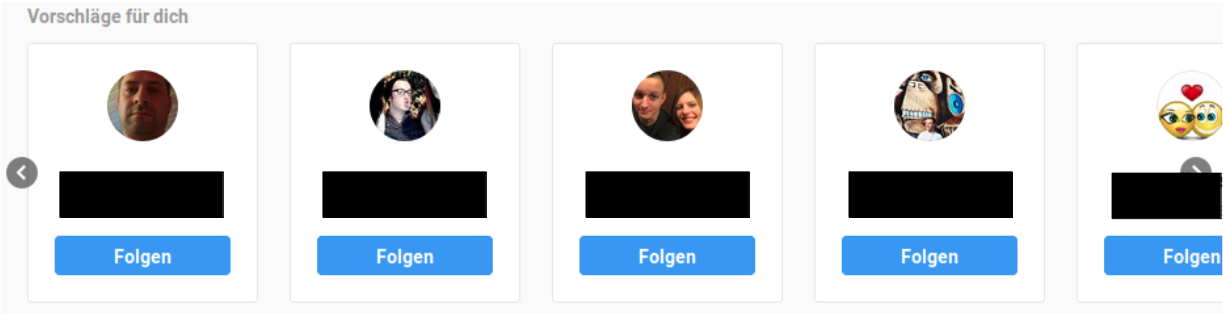
\includegraphics[ scale=0.35]{bilder/instagram_vorschlaege.png}
			\caption{Container mit Profil-Vorschlägen}
			\label{img:instagram_vorschlaege}
		\end{figure}
		
		Falls es sich um ein öffentlich frei zugängliches Profil handelt, kann eine Liste der abonnierten Kontakte angezeigt werden. Hierbei handelt es sich um ein scrollbares Pop-Up-Fenster \ref{img:instagram_abonniert}. Vergleichbar zur Methode bei einer privaten Profilseite, wird hier ebenfalls Schritt-für-Schritt durchgescrollt. Dadurch wird jedes einzelne Profil geladen und der dazugehörig Link, zur dieser Profilseite, kann dadurch ausgelesen werden. 
		
		
		
		\begin{figure}[H]
			\centering
			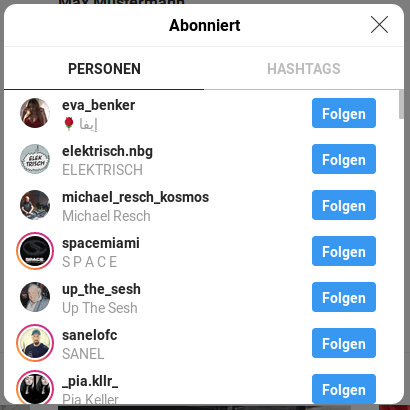
\includegraphics[ scale=0.35]{bilder/instagram_abonniert.png}
			\caption{Pop-up-Fenster mit abonnierten Profilen}
			\label{img:instagram_abonniert}
		\end{figure}
	
		Die Herausforderung besteht darin, dass nicht zu schnell gescrollt werden darf. Aus diesem Grund wird ein Algorithmus \ref{lst:AlgoZumDurchscrollen} verwendet, welcher einem menschlichen Verhalten ähneln soll. Hierbei wird zuallererst das Pop-up-Fenster gesucht und festgelegt. Anschließend wir die Anzahl der abonnierten Profile gezählt. Die Anzahl der Profile wird dazu verwendet, dass der Algroithmus weiß wie weit nach unten geblättert werden muss, um alle Profil zu laden.\\
		Im ersten Schritt, wird das Fenster nur ein sechstel des möglichen Bereichs nach unten gescrollt. Dadurch werden weitere Profile geladen. Wenn direkt nach ganz unten geblättert wird, wäre dies beim ersten Scrollvorgang zu schnell. In diesem Fall werden keine Kontakte geladen. Es werden lediglich Profil von sehr bekannten Instagram-Usern angezeigt, die von dieser Person abonniert wurden.\\
		In den nächsten Schritte wird das Fenster jeweils ganz nach unten verschoben. Dadurch werden alle Profile geladen. Sobald alle Links bekannt sind, wird eine URL zu den entsprechenden Profilseiten erstellt. Diese Seiten werden anschließen wie jede andere Seite ausgelesen und nach Information durchsucht. Infolgedessen wird die gewonnene Information jedes Profils mit der Information der Zielperson verglichen. Die Suche wird bei einem beliebigen Treffer beendet. Anschließend wird die gefunden Information mit dem Namen des Benutzers der Profilseite gespeichert. Diese abgespeicherten Daten können später zur E-Mail-Generierung verwendet werden.\\
		
		\begin{lstlisting}[caption=Herunterscrollen des Pop-up Fensters,label={lst:AlgoZumDurchscrollen}]
			# Find the pop-up window
			pop_up = self.browser.find_element_by_xpath('/html/body/div[2]
					/div/div[2]')        
			# find number of followers
			all_following = int(self.browser.find_element_by_xpath("//li[2]
					/a/span").text)
			# scroll down the page
			for i in range(int(all_following / 6)):
				if i == 0:
					self.browser.execute_script("arguments[0].scrollTop = 
							arguments[0].scrollHeight/5", pop_up)
					time.sleep(2)
				else:
					self.browser.execute_script("arguments[0].scrollTop = 
							arguments[0].scrollHeight", pop_up)
				time.sleep(random.randint(500, 1000) / 1000)
		\end{lstlisting}



\section{Speicherung der gewonnenen Daten}
Die gespeicherten Daten werden von verschiedenen Klassen benötigt. Aus diesem Grund muss es möglich sein, dass andere Klassen auf die Speicherstruktur zugreifen können. Des Weiteren wird eine gute Struktur vorausgesetzt, damit auf einzelne Attribute der Person zugegriffen werden kann. Es ist nicht notwendig, dass die Daten nach Programmende abrufbar sind. Infolgedessen wird keine externe Speicherung in einer Datenbank oder in einer Datei vorausgesetzt.\\
Eine mögliche Speicherung der Daten wäre in einer SQL-Datenbank. Alternativ könnten die Personendaten in einer externen Datei oder mit Hilfe einem Personenobjekt gespeichert werden.\\
Eine SQL-Datenbank bringt eine gute Speicherstruktur mit sich. Allerdings sind mit einer SQL-Datenbank aufwendigere Speicher-und Abrufvorgänge verbunden. Die externe Speicherung in einer Datei wie CVS oder TXT ist keine Anforderung. Auf eine SQL-Datenbank sowie auf eine externe Datei, lässt sich mit jeder Klasse darauf zugegriffen. Dennoch wird ein Personenobjekt verwendet. Dadurch werden keine unnötigen Speicher- und Lesezugriffe benötigt. Darüber hinaus lässt sich das Personenobjekt an die entsprechenden Klassen übergeben.
	\subsection{Implementierung der Personenklasse}
	Die gewonnenen Daten werden in einem Personenobjekt, wie in Listing \ref{lst:AlgoPersonobject} dargestellt, gespeichert. Dabei werden die vom Anwender eingegebenen Daten direkt in das Personenobjekt übertragen. Die gewonnen Informationen werden in Form einer Liste hinzugefügt. Falls bei der Kontaktanalyse ein Treffer gemacht wurde, kann diese Information in dem Attribute "'contacts\_information gespeichert werden. Hierbei wird zuerst der vollständige Kontaktname und anschließend die übereinstimmende Information gespeichert. Ein Beispiel hierfür wäre ["'Max Mustermann"',"'Fußball"']\\
	
	\begin{lstlisting}[caption=Personklasse,label={lst:AlgoPersonobject}]
	class Person(object):
		def __init__(self):
			self.first_name = input("Vorname: ")
			self.second_name = input("Nachname: ")
			self.place_of_residence = input("Wohnort: ")
			self.year_of_birth = input("Geburtsjahr: ")
			self.institution = input("Institution: ")
			self.instagram_name = input("Instagram Benutzername: ")
			self.facebook_name = input("Facebook Benutzername: ")
			self.twitter_name = input("Twitter Benutzername: ")
			self.input_email = input("E-Mail-Adresse: ")
			self.occupation = []
			self.hobbies = []
			self.universities = []
			self.founded_mails = []
			self.locations = []
			self.contacts_information = []
	\end{lstlisting}
	
	